% ************************************************************************
% A Thesis Template
% for the Department of Mathematics, University of Toronto
% Copyright (C) 2019 Fabian Parsch
%
% This template is based on, and the vast majority of credit goes to
%
% A Classic Thesis Style v4.6
% An Homage to The Elements of Typographic Style
% Copyright (C) 2018 André Miede and Ivo Pletikosić 
%
% Please see the file ClassicThesis.pdf for more information.
% Your comments are highly appreciated.
%
% If you like the style then the authors of Classic Thesis would
% appreciate a postcard. Their address can be found in the file
% ClassicThesis.pdf. A collection of postcards they received so far
% is available online at http://postcards.miede.de
%
% License:
% This program is free software; you can redistribute it and/or modify
% it under the terms of the GNU General Public License as published by
% the Free Software Foundation; either version 2 of the License, or
% (at your option) any later version.
%
% This program is distributed in the hope that it will be useful,
% but WITHOUT ANY WARRANTY; without even the implied warranty of
% MERCHANTABILITY or FITNESS FOR A PARTICULAR PURPOSE.  See the
% GNU General Public License for more details.
%
% You should have received a copy of the GNU General Public License
% along with this program; see the file COPYING.  If not, write to
% the Free Software Foundation, Inc., 59 Temple Place - Suite 330,
% Boston, MA 02111-1307, USA.
% ************************************************************************

% This template is mostly a simplified and rearranged version of ClassicThesis v4.6
% https://ctan.org/pkg/classicthesis
% You are encouraged to check out ClassicThesisManual.pdf

% Besides simplifications, some slight adjustments were made to fulfill the University of Toronto School of Graduate Studies style requirements. It also includes some adjustments for better integration with the ams packages and for letter sized paper.


% The following four lines are necessary due to compatibility issues. They are suppressing some errors.
\RequirePackage{silence}
\WarningFilter{scrreprt}{Usage of package `titlesec'}
\WarningFilter{scrreprt}{Activating an ugly workaround}
\WarningFilter{titlesec}{Non standard sectioning command}

% You can run this document two ways.

% Option 1: Same margins on both sides and no "open right"
% This is the best option for the digital version of your thesis.
\documentclass[oneside,numbers=noenddot,headinclude,footinclude,cleardoublepage=empty,abstract=on,BCOR=5mm,paper=letter,fontsize=11pt]{scrreprt}

% Option 2: When you print your thesis, comment the above documentclass and uncomment the one below.
% The only difference is ``twoside'' instead of ``oneside''
% That way, the outer margins are larger than the inner margins. Also, chapters are always opened on the right hand side.
% This results in a MUCH nicer printed version. No worries, all page breaks remain where they are, it just moves everything to the left or right a bit.
% ALSO: Make sure to uncomment the addmargin environments in titlepage.tex and colophon.tex. That way, the first and last page remain centered
%\documentclass[twoside,numbers=noenddot,headinclude,footinclude,cleardoublepage=empty,abstract=on,BCOR=5mm,paper=letter,fontsize=11pt]{scrreprt}

% So to recap: Typeset your whole thesis with Option 1 and submit the resulting version electronically
% But before actually printing the thesis, rerun the document with Option 2.

% Any packages, newcommands, ... should be put in the thesisconfig file.
% This is the file where all your settings, packages, newcommands, ... should go

\PassOptionsToPackage{T1}{fontenc}
  \usepackage{fontenc}

% Configure classicthesis for your needs here.
% (see ClassicThesis.pdf for more information)
\PassOptionsToPackage{
  drafting=false,    % print version information on the bottom of the pages
  tocaligned=false, % the left column of the toc will be aligned (no indentation)
  dottedtoc=true,  % page numbers in ToC flushed right
  eulerchapternumbers=true, % use AMS Euler for chapter font (otherwise Palatino)
  linedheaders=false,       % chaper headers will have line above and beneath
  floatperchapter=true,     % numbering per chapter for all floats (i.e., Figure 1.1)
  eulermath=false,  % use awesome Euler fonts for mathematical formulae (only with pdfLaTeX)
  beramono=true,    % toggle a nice monospaced font (w/ bold)
  palatino=false,    % deactivate standard font for loading another one, see the last section at the end of this file for suggestions
  parts=false,
  style=classicthesis
}{classicthesis}

% Personal data (insert your own data here)
\newcommand{\myTitle}{Computing the generating function of a coinvariants map\xspace}
\newcommand{\myName}{Jesse Frohlich\xspace}
\newcommand{\myDegree}{Doctor of Philosophy\xspace}
\newcommand{\myDepartment}{Graduate Department of Mathematics\xspace}
\newcommand{\myUni}{University of Toronto\xspace}
\newcommand{\myTime}{2023\xspace}

% Load all the packages you want here
% Probably you will need the following
\PassOptionsToPackage{english}{babel}
\usepackage{fontsetup}
\usepackage{babel} % language support
\usepackage{enumitem} % for better itemize and enumerate
\usepackage{mathtools,amsthm,amssymb} % because math
\usepackage{mleftright}
\usepackage{etoolbox}
\usepackage{thmtools} % for correct autorefs
\usepackage[onehalfspacing]{setspace} % as required by SGS
\usepackage{graphicx} % to include graphics
\usepackage{xspace} % to get the spacing after macros right
\usepackage{calc} % to allow adding lengths
\usepackage{multicol}
\usepackage{ulem}
\usepackage{stmaryrd}
\usepackage{acronym}
\usepackage{newunicodechar}
\usepackage{ltablex}
\usepackage{ragged2e}
\usepackage{pdflscape}

\usepackage[langlinenos=true]{minted}
\setminted{breaklines=true,linenos=true}
\setminted[mathematica]{firstnumber=last}
\usemintedstyle[wolfram]{mathematica}
\newminted[code]{haskell}{firstnumber=last}
\newminted[spec]{haskell}{}
\newmintinline[hs]{haskell}{}
\newmintinline[mma]{mathematica}{}

% Theorem-like environments

        \ProvideDocumentCommand{\defi}{m}{\uline{#1}} % Item being DEFined

        \newcommand{\alignedintertext}[1]{%
          \noalign{%
            \vskip\belowdisplayshortskip
            \vtop{\hsize=\linewidth#1\par
            \expandafter}%
            \expandafter\prevdepth\the\prevdepth
          }%
        }

% Font changes

        \ProvideDocumentCommand{\mcl}{m}{\mathcal{#1}}
        \ProvideDocumentCommand{\mbb}{m}{\mathbb{#1}}
        \ProvideDocumentCommand{\mbf}{m}{\boldsymbol{\mathbf{#1}}}
        \ProvideDocumentCommand{\msc}{m}{\mathscr{#1}}
        \ProvideDocumentCommand{\mfk}{m}{\mathfrak{#1}}
        \ProvideDocumentCommand{\mit}{m}{\mathit{#1}}

% Symbols

        \ProvideDocumentCommand{\lt}{}{<}
        \ProvideDocumentCommand{\gt}{}{>}
        \ProvideDocumentCommand{\eq}{}{=}
        \ProvideDocumentCommand{\defeq}{}{\coloneq}
        \newcommand{\iso}{\cong} % or \cong
        \newcommand{\homeo}{\cong} % or \cong
        \newcommand{\hty}{\cong} % or \cong
        \ProvideDocumentCommand{\then}{}{\mathbin{/\mkern-6mu/}}
        \newcommand{\fracl}[2]{\left.{#1}\middle/{#2}\right.}
        \renewcommand{\boundary}{\partial}
        \newunicodechar{∂}{\ensuremath\partial}
        \newunicodechar{⋯}{\ensuremath\cdots}
        \newunicodechar{⋮}{\ensuremath\vdots}
        \newunicodechar{…}{\ensuremath\dots}

% Standard number sets.
        \newcommand{\N}{\mbb{N}}   % Natural
        \newcommand{\Z}{\mbb{Z}}   % Integer
        \newcommand{\Q}{\mbb{Q}}   % Rational
        \newcommand{\R}{\mbb{R}}   % Real
        \newcommand{\C}{\mbb{C}}   % Complex
        \newcommand{\F}{\mbb{F}}   % Finite
        \newcommand{\K}{\mbb{k}}   % Generic

% Common operators

        \ProvideDocumentCommand{\inv}{sm}{% Invert something
                \IfBooleanTF{#1}
                        {\frac1{#2}}
                        {#2^{-1}}
        }
        % Exponential Map
        \ProvideDocumentCommand{\Exp}{m}{%
                \mbf e^{#1}
        }
        \ProvideDocumentCommand{\invb}{m}{\overline{#1}} % bar-style inverse
        \DeclareMathOperator{\dom}{dom}        % Domain
        \DeclareMathOperator{\cod}{cod}        % Codomain
        \ProvideDocumentCommand{\id}{o}{
          \IfNoValueTF {#1}
            {\operatorname{id}}
            {\operatorname{id}_{#1}}
        }
        \ProvideDocumentCommand{\Id}{m}{\id^{#1}_{#1}}
        \ProvideDocumentCommand{\dual}{m}{{#1}^*}

        \DeclareMathOperator{\Span}{span}       % span
        \DeclareMathOperator{\nullity}{nullity} % nullity
        \DeclareMathOperator{\rank}{rank}       % rank
        \DeclareMathOperator{\trace}{tr}        % trace
        \DeclareMathOperator{\Null}{Null}      % Nullspace
        \DeclareMathOperator{\Gal}{Gal}        % Galois group
        \DeclareMathOperator{\Spec}{Spec}      % Spectrum
        \DeclareMathOperator{\Frac}{Frac}      % Field of fractions
        \DeclareMathOperator{\Proj}{Proj}      % Proj construction
        \DeclareMathOperator*{\esssup}{ess\,sup} % essential supremum
        \DeclareMathOperator*{\supp}{supp}     % support
        \ProvideDocumentCommand{\centre}{}{%
          Z
          % ζ
        }

        \ProvideDocumentCommand{\Operator}{moo}{
          \IfNoValueTF{#2}
            {#1}
            {\IfNoValueTF{#3}% Don't make parentheses expand beyond the operator.
              {#1_{#2}}
              {#1_{#2}^{#3}}
              % {\vphantom{#1^{-}}\smash{#1_{#2}}}
              % {\vphantom{#1^{-}}\smash{#1_{#2}^{#3}}}
            }
        }


        % There should really be another argument for what the operator is acting on,
        % but that's a lot more typing I really don't care to do. However, semantically
        % this is the way to go, and snippets *are* at my disposal.
        % {oo} means "take two optional arguments"
        \ProvideDocumentCommand{\Sum   }{oo}{\Operator\sum      [#1][#2]}
        \ProvideDocumentCommand{\Dsum  }{oo}{\Operator\bigoplus [#1][#2]}
        % The following code does not work. Why is this?
        \ProvideDocumentCommand{\Dsumc }{oo}{\Operator{\bigoplus}[#1][#2]}
        \ProvideDocumentCommand{\Prod  }{oo}{\Operator\prod     [#1][#2]}
        \ProvideDocumentCommand{\Tprod }{oo}{\Operator\bigotimes[#1][#2]}
        \ProvideDocumentCommand{\Coprod}{oo}{\Operator\coprod   [#1][#2]}
        \ProvideDocumentCommand{\Dunion}{oo}{\Operator\bigsqcup [#1][#2]}
        \ProvideDocumentCommand{\Union }{oo}{\Operator\bigcup   [#1][#2]}
        \ProvideDocumentCommand{\Inter }{oo}{\Operator\bigcap   [#1][#2]}
        \ProvideDocumentCommand{\Int   }{oo}{\Operator\int      [#1][#2]}
        \newcommand{\gint}{\mathrlap{\int}\,G}
        \ProvideDocumentCommand{\GInt  }{}{\Operator\gint     }
        \ProvideDocumentCommand{\IInt  }{oo}{\Operator\iint     [#1][#2]}
        \ProvideDocumentCommand{\IIInt }{oo}{\Operator\iiint    [#1][#2]}
        \ProvideDocumentCommand{\Wedge }{oo}{\Operator\bigwedge [#1][#2]}

% Rings

        \ProvideDocumentCommand{\polyring}{mm}{#1\bk{#2}}
        \ProvideDocumentCommand{\powerseries}{mm}{#1\bkk{#2}}

% Classic Groups
        \DeclareMathOperator{\GL}{GL}
        \DeclareMathOperator{\SL}{SL}
        \DeclareMathOperator{\SP}{Sp}
        \DeclareMathOperator{\SO}{SO}
        \DeclareMathOperator{\Spin}{Spin}
        \DeclareMathOperator{\U}{U}
        \DeclareMathOperator{\SU}{SU}
        \DeclareMathOperator{\Or}{O}

% Lie algebras

        %% Algebras

                \DeclareMathOperator{\Gl}{\mfk{gl}}
                \DeclareMathOperator{\Sp}{\mfk{sp}}
                \DeclareMathOperator{\Sl}{\mfk{sl}}
                \DeclareMathOperator{\So}{\mfk{so}}
                \DeclareMathOperator{\g}{\mfk{g}}
                \newcommand{\fg}{\mfk{g}}
                \newcommand{\fh}{\mfk{h}}
                \newcommand{\fn}{\mfk{n}}
                \newcommand{\fb}{\mfk{b}}

        %% Lie algebra operations

                \DeclareMathOperator{\ad}{ad}   % adjoint
                \DeclareMathOperator{\Ad}{Ad}   % Big Adjoint
                \DeclareMathOperator{\Lie}{Lie} % Lie algebra

        %% Universal enveloping algebra
                \ProvideDocumentCommand{\uea}{sO{}m}{
                        \mathfrak{
                                \IfBooleanTF{#1}{\hat U}{U}
                        }_{#2}\pn{#3}
                }

% Categories
        \ProvideDocumentCommand{\catname}{m}{\mathbf{#1}}
        \DeclareMathOperator{\mfld  }{\catname{Mfld}}
        \DeclareMathOperator{\mfldb }{\catname{Mfld}\pmb\boundary}
        \DeclareMathOperator{\Vect  }{\catname{Vect}}
        \DeclareMathOperator{\Mod   }{\catname{Mod}}
        \DeclareMathOperator{\Set   }{\catname{Set}}
        \DeclareMathOperator{\Ring  }{\catname{Ring}}
        \DeclareMathOperator{\Top   }{\catname{Top}}
        \DeclareMathOperator{\FinSet}{\catname{FinSet}}

% Paired Delimiters

\ProvideDocumentCommand{\curry}{m}{\ifblank{#1}{\:\cdot\:}{#1}}

%% Parenthetical constructs
\DeclarePairedDelimiter{\pn}\lparen\rparen
\DeclarePairedDelimiter{\set}\{\}
\DeclarePairedDelimiter{\bk}\lbrack\rbrack
\DeclarePairedDelimiter{\bkk}\llbracket\rrbracket
\DeclarePairedDelimiter{\gen}\langle\rangle

%% Operators

\DeclarePairedDelimiterX{\commutator}[2]{[}{]}{\curry{#1}, \curry{#2}}

\DeclarePairedDelimiterX{\liebk}[2]{[}{]}{\curry{#1}, \curry{#2}}

\DeclarePairedDelimiterXPP{\normHelper}[2]{}\lVert\rVert
        {\IfNoValueTF{#2}{}{_{#2}}}
        {\curry{#1}}
\ProvideDocumentCommand{\norm}{s O{} m o}{% Optional subscript token at the end.
        \IfBooleanTF{#1}
                {\normHelper*{#3}{#4}}
                {\normHelper[#2]{#3}{#4}}
}

\DeclarePairedDelimiterXPP{\absHelper}[2]{}\lvert\rvert
        {\IfNoValueTF{#2}{}{_{#2}}}
        {\curry{#1}}
\ProvideDocumentCommand{\abs}{s O{} m o}{% Optional subscript token at the end.
        \IfBooleanTF{#1}
                {\absHelper*{#3}{#4}}
                {\absHelper[#2]{#3}{#4}}
}

\NewDocumentCommand{\restrict}{sO{}mO{}}{%
        \IfBooleanTF{#1}{% star
                \mleft.\kern-\nulldelimiterspace
                #3
                \mright|%
        }{% no star
                #3#2|%
        }%
        _{#4}%
}

\DeclarePairedDelimiterX{\pair}[2]\langle\rangle{%
        \nonscript\,\curry{#1}\PairSymbol[\delimsize]{\vert}\curry{#2}\nonscript\,%
}

\DeclarePairedDelimiterX{\inner}[2]\langle\rangle{%
        \nonscript\,\curry{#1}\PairSymbol[\delimsize]{,}\curry{#2}\nonscript\,%
}

\DeclarePairedDelimiterXPP{\contractionHelper}[2]{}\langle\rangle
        {\IfNoValueTF{#2}{}{_{#2}}}
        {\curry{#1}}
\ProvideDocumentCommand{\contraction}{s O{} m o}{% Optional subscript token at the end.
        \IfBooleanTF{#1}
                {\contractionHelper*{#3}{#4}}
                {\contractionHelper[#2]{#3}{#4}}
}

\DeclarePairedDelimiterX{\card}[1]\lvert\rvert{\curry{#1}}
% \ProvideDocumentCommand{\card}{\#}

\DeclarePairedDelimiterX\ceil [1]{\lceil}{\rceil}{\curry{#1}}

\DeclarePairedDelimiterX\floor[1]{\lfloor}{\rfloor}{\curry{#1}}

\DeclarePairedDelimiterX\ord  [1]{\lvert}{\rvert}{\curry{#1}}
\DeclareMathOperator{\Ord}{ord}


%% Building constructs

% can be useful to refer to this outside \Set
\ProvideDocumentCommand{\innerspacing}{}{\mathchoice{\:}{\:}{\,}{\,}}
\newcommand\SetSymbol[1][]{%
  \innerspacing%
  %:%
  #1\vert%
  \allowbreak\innerspacing\mathopen{}%
}
\newcommand\PairSymbol[2][]{%
  \nonscript\, #1 #2 \allowbreak\nonscript\,\mathopen{}%
}

\DeclarePairedDelimiterX{\setbuilder}[2]\{\}{\,#1\SetSymbol[\delimsize]#2\,}

\DeclarePairedDelimiterX{\genbuilder}[2]\langle\rangle{\,#1\SetSymbol[\delimsize]#2\,}

\newcommand{\grppres}{\genbuilder}

\DeclareMathOperator{\Object}{Ob} 
\DeclareMathOperator{\HomOp}{Hom} 
\DeclarePairedDelimiterXPP{\HomHelper}[3]
        {\IfNoValueTF{#1}
                {\HomOp}
                {\HomOp_{#1}}
        }
        ()
        {}{\curry{#2}, \curry{#3}}
\ProvideDocumentCommand{\Hom}{s O{} m m}{
        \IfBooleanTF{#1}
                {\HomHelper*{#2}{#3}{#4}}
                {\HomHelper{#2}{#3}{#4}}
}

% Maps
        \ProvideDocumentCommand{\map}{mmO{\to}m}{#1\colon#2#3#4}
        \ProvideDocumentCommand{\nodomainmap}{mmm}{#1\colon#2\mapsto#3}
        \ProvideDocumentCommand{\selfmap}{mmO{\to}}{#1\colon#2#3#2}
        \ProvideDocumentCommand{\selfmapdef}{mmO{\to}m m }{%
                \begin{aligned}
                        #1\colon#2&#3#2\\
                        #4&\mapsto#5
                \end{aligned}%
        }
        \ProvideDocumentCommand{\mapdef}{mmO{\to}m m m o}{%
                \begin{aligned}
                        #1\colon#2&#3#4\\
                        #5&\mapsto#6
                        \IfNoValueTF{#7}{}{\\ #7}
                \end{aligned}%
        }

        \newcommand{\mono}{\hookrightarrow} % monomorphism
        \newcommand{\inc }{\hookrightarrow} % inclusion % DEPRECATE?
        \newcommand{\inj }{\hookrightarrow} % injection
        \newcommand{\emb }{\hookrightarrow} % embedding
        \newcommand{\sur }{\twoheadrightarrow} % epimorphism
        \newcommand{\epi }{\twoheadrightarrow} % epimorphism
        \newcommand{\toiso }{\xrightarrow{\sim}} % isomorphism

% Quantum groups / Hopf algebras

\newcommand{\unit}{\eta}           % unit
\newcommand{\one}{\mbf 1}          % another form of the unit
\newcommand{\counit}{\epsilon}     % counit

\newcommand{\mult}{m}              % multiplication
\newcommand{\comult}{\Delta}       % comultiplication
\ProvideDocumentCommand{\cmf}{mm}  % comultiplication factor
  {#2_{(#1)}}

\newcommand{\antipode}{S}          % antipode
\ProvideDocumentCommand{\bap}{m}   % bar-antipode
  {\overline{#1}}
\ProvideDocumentCommand{\baap}{m}  % bar-inverse(i.e. anti)-antipode
  {\underline{#1}}

\newcommand{\rmat}{r}         % Lie-algebraic r-matrix

\newcommand{\Rmat}{\mcl R}         % R-matrix
\newcommand{\Rmati}{\invb\Rmat}
\ProvideDocumentCommand{\rmf}{O{}} % R-matrix First factor
  {\Rmat^{(1)}_{#1}}
\ProvideDocumentCommand{\rms}{O{}} % R-matrix Second factor
  {\Rmat^{(2)}_{#1}}

\ProvideDocumentCommand{\coevf}{m} % Coevaluation First factor
  {r_{#1}}
\ProvideDocumentCommand{\coevd}{m} % Coevaluation Dual factor
  {ρ_{#1}}

\ProvideDocumentCommand{\spin}{}{C}
\ProvideDocumentCommand{\ribbon}{}{ν}
\ProvideDocumentCommand{\dfe}{}{\mfk u}
\ProvideDocumentCommand{\monodromy}{}{Q}

% Thesis-specific macros

\ProvideDocumentCommand{\ptr}{}{Z^\trace}
\ProvideDocumentCommand{\fa}{}{\mfk{a}}
\ProvideDocumentCommand{\Alg}{}{\fg}
\ProvideDocumentCommand{\CUlong}{}{\uea*{\Sl_{2+}^0}}
\ProvideDocumentCommand{\CU}{}{U}
\ProvideDocumentCommand{\nn}{}{\mathbf{n}}
\ProvideDocumentCommand{\Order}{}{\mathbb O}
\RenewDocumentCommand{\k}{}{\mbf k}
\DeclareMathOperator{\GenMap}{\msc G} 
\DeclarePairedDelimiterXPP{\Gen}[1]{\GenMap}\lparen\rparen{}{#1}
\ProvideDocumentCommand{\tangle}{}{\msc T}
\ProvideDocumentCommand{\RVT}{}{\msc{T}^{\text{rv}}}
\ProvideDocumentCommand{\A}{}{\msc{A}}
\ProvideDocumentCommand{\tanglename}{momm}{#1_{
                #3%
                \IfValueTF{#2}{\text{#2}}{,}%
                #4
}}
\newcommand{\knot}{\tanglename{K}} 
\newcommand{\link}{\tanglename{L}} 


% Her Majesty herself
\usepackage{classicthesis}

% Fine-tune hyperreferences (hyperref should be called last)
\hypersetup{%
  %draft, % hyperref's draft mode, for printing see below
  colorlinks=true, linktocpage=true, pdfstartpage=3, pdfstartview=FitV,%
  % uncomment the following line if you want to have black links (e.g., for printing)
  %colorlinks=false, linktocpage=false, pdfstartpage=3, pdfstartview=FitV, pdfborder={0 0 0},%
  breaklinks=true, pageanchor=true,%
  pdfpagemode=UseNone, %
  % pdfpagemode=UseOutlines,%
  plainpages=false, bookmarksnumbered, bookmarksopen=true, bookmarksopenlevel=1,%
  hypertexnames=true, pdfhighlight=/O,%nesting=true,%frenchlinks,%
  urlcolor=CTurl, linkcolor=CTlink, citecolor=CTcitation, %pagecolor=RoyalBlue,%
  %urlcolor=Black, linkcolor=Black, citecolor=Black, %pagecolor=Black,%
  pdftitle={\myTitle},%
  pdfauthor={\textcopyright\ \myName, \myDepartment, \myUni},%
  pdfsubject={},%
  pdfkeywords={},%
  pdfcreator={pdfLaTeX},%
  pdfproducer={LaTeX with hyperref and classicthesis}%
}
\usepackage[noabbrev]{cleveref}

% Setup autoreferences (hyperref and babel)
% In the document, don't use \ref{...}
% Instead, use \autoref{...}
% That changes the reference from "3.1" to "Definition 3.1"
\makeatletter
\@ifpackageloaded{babel}%
  {%
    \addto\extrasenglish{%
      \renewcommand*{\figureautorefname}{Figure}%
      \renewcommand*{\tableautorefname}{Table}%
      \renewcommand*{\partautorefname}{Part}%
      \renewcommand*{\chapterautorefname}{Chapter}%
      \renewcommand*{\sectionautorefname}{Section}%
      \renewcommand*{\subsectionautorefname}{Section}%
      \renewcommand*{\subsubsectionautorefname}{Section}%
      \renewcommand*{\theoremautorefname}{Theorem}%
      \renewcommand*{\lemmaautorefname}{Lemma}%
      \renewcommand*{\conjectureautorefname}{Conjecture}%
      \renewcommand*{\corollaryautorefname}{Corollary}%
      \renewcommand*{\definitionautorefname}{Definition}%
      \renewcommand*{\methodautorefname}{Method}%
      \renewcommand*{\factautorefname}{Fact}%
      \renewcommand*{\problemautorefname}{Problem}%
      \renewcommand*{\questionautorefname}{Question}%
      \renewcommand*{\exampleautorefname}{Example}%
      \renewcommand*{\remarkautorefname}{Remark}%    
    }%
    }{\relax}
\makeatother

% This changes the regular classicthesis chapter header to one that is a bit larger and uses red as a colour
\makeatletter
\ifthenelse{\boolean{ct@linedheaders}}%
{% lines above and below, number right
    \titleformat{\chapter}[display]%
    {\relax}{\raggedleft{\color{CTsemi}\chapterNumber\thechapter} \\ }{0pt}%
    {\titlerule\vspace*{.9\baselineskip}\raggedright\Large\color{CTtitle}\spacedallcaps}[\normalsize\vspace*{.8\baselineskip}\titlerule]%
}{% something like Bringhurst
    \titleformat{\chapter}[display]%
    {\relax}{\mbox{}\oldmarginpar{\vspace*{-3\baselineskip}\color{CTsemi}\chapterNumber\thechapter}}{0pt}%
    {\raggedright\huge\color{CTtitle}\spacedallcaps}[\normalsize\vspace*{.8\baselineskip}\titlerule]%
}
\makeatother

% Load tikz-cd after chapter title redefinition.
\usepackage{tikz-cd}
\usepackage{csquotes}

% Add any other environments you might need here
% Note: You should also add any new environments to the autorefnames above
\newtheorem{theorem}{Theorem}[chapter]
\newtheorem{lemma}[theorem]{Lemma}
\newtheorem{conjecture}[theorem]{Conjecture}
\newtheorem{corollary}[theorem]{Corollary}

\theoremstyle{definition}
\newtheorem{definition}[theorem]{Definition}
\newtheorem{method}[theorem]{Method}
\newtheorem{fact}[theorem]{Fact}
\newtheorem{problem}[theorem]{Problem}
\newtheorem{question}[theorem]{Question}
\newtheorem{example}[theorem]{Example}

\theoremstyle{remark}
\newtheorem{remark}[theorem]{Remark}

% Better spacing than regular itemize
\newenvironment{itemize*}
  {\begin{itemize}[topsep=-\parskip+\jot,itemsep=-\parskip-\jot]}
  {\end{itemize}}
  
% Better spacing than regular enumerate, (a), (b), ...
\newenvironment{enumerate*}
  {\begin{enumerate}[label=(\alph*),topsep=-\parskip+\jot,itemsep=-\parskip-\jot]}
  {\end{enumerate}}
  
% Better spacing than regular enumerate, (i), (ii), ...
\newenvironment{enumerate**}
  {\begin{enumerate}[label=(\roman*),topsep=-\parskip+\jot,itemsep=-\parskip-\jot]}
  {\end{enumerate}}
  
% Better spacing than regular enumerate, (a'), (b'), ...
\newenvironment{enumerate***}
  {\begin{enumerate}[label=(\alph*'),topsep=-\parskip+\jot,itemsep=-\parskip-\jot]}
  {\end{enumerate}}


\begin{document}

% If you are wondering what \frenchspacing does, check out the Internet then decide if you want to use it.
\frenchspacing
\raggedbottom

\selectlanguage{english}

% Frontmatter
% Note: SGS requires that the abstract is on the second page. Do not move it further down.
% Roman page numbering is also required by SGS.
\pagenumbering{roman}
\pagestyle{plain}
% Do NOT edit the title info here. There is a central place to set Title, Author etc. in thesisconfig.tex
\begin{titlepage}
    \pdfbookmark[1]{\myTitle}{titlepage}

% Uncomment the addmargin environment when using Option 2 in the main file
% \begin{addmargin}[-0.6cm]{-3cm}
    \begin{center}
        \large

        \hfill

        \vfill

        \begingroup
            \color{CTtitle}\spacedallcaps{\myTitle}
        \endgroup

		\vfill
		\spacedlowsmallcaps{by}\bigskip
		
        \spacedlowsmallcaps{\myName}

		\vfill
        
        A thesis submitted in conformity with\\
        the requirements for the degree of\smallskip
        
        \myDegree \smallskip
        
        \myDepartment\\
        \myUni\bigskip
        
        \textcopyright\ \myTime \myName

    \end{center}
% \end{addmargin}
\end{titlepage}

\cleardoublepage
\pdfbookmark[1]{Abstract}{Abstract}

\begingroup
\let\clearpage\relax
\let\cleardoublepage\relax
\let\cleardoublepage\relax

\chapter*{Abstract}

\doublespacing

% Do NOT edit the title info here. There is a central place to set Title, Author etc. in the thesisconfig.tex
\begin{center}
	\myTitle\\
\myName\\
\myDegree\\
\myDepartment\\
\myUni\\
\myTime
\end{center}

A well-known source of strong link invariants comes from quantum groups.
Typically, one uses a representation of a quantum group to build a computable
invariant, though these computations require exponential time in the number of
crossings. Recent work has allowed for direct and efficient computations within
the quantum groups themselves, through the use of perturbed Gaußian
differential operators. This thesis introduces and explores a partial expansion
of the tangle-theoretic computations performed by Bar-Natan and van der Veen
\cite{BV} in the quantum group $\uea{\Sl_{2+}^0}$ to its space of coinvariants,
providing an extension of this computational method from open tangles to links.
We compute a basis for the space of coinvariants, then compute a closed-form
expression for the corresponding trace map in the form of a generating function.
The resulting function is not a compatible perturbed Gaußian with respect to the
previous research, so in addition, we find a method of computing the link
invariant for a subclass of links. After writing a program to compute the
invariant on two-component links, we found unexpectedly that this extension is
neither stronger nor weaker than the \acl{MVA}. 
\endgroup

\cleardoublepage
\phantomsection
\pdfbookmark[1]{Dedication}{Dedication}

\vspace*{3cm}

\begingroup
\setlength{\parindent}{0cm}
\textit{To someone,\\
\hspace*{5mm}who did something nice.}
\endgroup


\cleardoublepage
\pdfbookmark[1]{Acknowledgements}{acknowledgements}

\begingroup
\let\clearpage\relax
\let\cleardoublepage\relax

\chapter*{Acknowledgements}

Lorem ipsum dolor sit amet, consetetur sadipscing elitr, sed diam nonumy eirmod tempor invidunt ut labore et dolore magna aliquyam erat, sed diam voluptua. At vero eos et accusam et justo duo dolores et ea rebum. Stet clita kasd gubergren, no sea takimata sanctus est Lorem ipsum dolor sit amet. Lorem ipsum dolor sit amet, consetetur sadipscing elitr, sed diam nonumy eirmod tempor invidunt ut labore et dolore magna aliquyam erat, sed diam voluptua. At vero eos et accusam et justo duo dolores et ea rebum. Stet clita kasd gubergren, no sea takimata sanctus est Lorem ipsum dolor sit amet. Lorem ipsum dolor sit amet, consetetur sadipscing elitr, sed diam nonumy eirmod tempor invidunt ut labore et dolore magna aliquyam erat, sed diam voluptua. At vero eos et accusam et justo duo dolores et ea rebum. Stet clita kasd gubergren, no sea takimata sanctus est Lorem ipsum dolor sit amet.   

Duis autem vel eum iriure dolor in hendrerit in vulputate velit esse molestie consequat, vel illum dolore eu feugiat nulla facilisis at vero eros et accumsan et iusto odio dignissim qui blandit praesent luptatum zzril delenit augue duis dolore te feugait nulla facilisi. Lorem ipsum dolor sit amet,


\endgroup

% The following command will make sure that publications are on the left and contents are on the right.
\cleardoubleevenpage
\pdfbookmark[1]{Publications}{publications}
\chapter*{Publications}

Here you can include a paragraph that links your thesis to your publications. For example you can point out that \autoref{ch:intro} is based on your publication \cite{gauss}.
\clearpage
\setlength{\cftbeforetoctitleskip}{100em}
\begingroup
\pagestyle{scrheadings}
\pdfbookmark[1]{\contentsname}{tableofcontents}
\setcounter{tocdepth}{1} % <-- 2 includes up to subsections in the ToC
\setcounter{secnumdepth}{1} % <-- 3 numbers up to subsubsections
\manualmark
\markboth{\spacedlowsmallcaps{\contentsname}}{\spacedlowsmallcaps{\contentsname}}
\tableofcontents
\automark[section]{chapter}
\renewcommand{\chaptermark}[1]{\markboth{\spacedlowsmallcaps{#1}}{\spacedlowsmallcaps{#1}}}
\renewcommand{\sectionmark}[1]{\markright{\textsc{\thesection}\enspace\spacedlowsmallcaps{#1}}}
\endgroup


% Add any chapters here
\cleardoublepage
\pagestyle{scrheadings}
\pagenumbering{arabic}
\cleardoublepage
\chapter{Differentiable Manifolds}
\label{ch:intro}

In mathematics, a differentiable manifold\footnote{also differential manifold} is a type of manifold that is locally similar enough to a linear space to allow one to do calculus. Any manifold can be described by a collection of charts, also known as an atlas. One may then apply ideas from calculus while working within the individual charts, since each chart lies within a linear space to which the usual rules of calculus apply.

\section{Topological Manifolds}

Here are two definitions.

\begin{definition}[Locally Euclidean Space]\label{def:locallyeuclidean}
A topological space $X$ is called \emph{locally Euclidean} if there is a non-negative integer $n$ such that every point in $X$ has a neighbourhood which is homeomorphic to $\mathbb{R}^n$
\end{definition}

\begin{definition}[Topological Manifold]\label{def:topman}
	A \emph{topological manifold} is a locally Euclidean Hausdorff space.
\end{definition}

\section{Differentiable Manifolds}

Now let's define something else.

\begin{definition}[Differentiable Manifold]\label{def:diffman}
	A \emph{differentiable manifold} is a topological manifold equipped with an equivalence class of atlases whose transition maps are all differentiable.
\end{definition}

\section{Main Theorem of This Thesis}

\begin{theorem}[Theorema Egregium]
	The Gaussian curvature of a surface is invariant under local isometry.
\end{theorem}

\begin{proof}
	This is immediate from \autoref{def:diffman}. Details are left as an exercise to the reader.
\end{proof}
\cleardoublepage
% Note that depending on your settings in the table of contents, subsections and subsubsections might appear virtually identical.
% Make sure to set the ToC depth and the numbering depth in the ToC the way you want.
\chapter{Examples}\label{ch:examples}
Ei choro aeterno antiopam mea, labitur bonorum pri no \cite{gauss}. His no decore nemore graecis. Suavitate interpretaris eu, vix eu libris efficiantur.

\section{A New Section}
Illo principalmente su nos. Non message \emph{occidental} angloromanic da. Debitas effortio simplificate sia se, auxiliar summarios da que, se avantiate publicationes via. Pan in terra summarios, capital interlingua se que. Al via multo esser specimen, campo responder que da. Le usate medical addresses pro, europa origine sanctificate nos se.

Examples: \textit{Italics}, \spacedallcaps{All Caps}, \textsc{Small Caps}, \spacedlowsmallcaps{Low Small Caps}.

Colours: \textcolor{CTtitle}{red}, \textcolor{CTcitation}{green}, \textcolor{CTlink}{blue}


\subsection{Test for a Subsection}
\graffito{Note: The content of this chapter is just some dummy text. It is not a real language.}
Lorem ipsum at nusquam appellantur his, ut eos erant homero concludaturque. Albucius appellantur deterruisset id eam, vivendum partiendo dissentiet ei ius. Vis melius facilisis ea, sea id convenire referrentur, takimata adolescens ex duo. Ei harum argumentum per. Eam vidit exerci appetere ad, ut vel zzril intellegam interpretaris.

Errem omnium ea per, pro con populo ornatus cu, ex qui dicant nemore melius. No pri diam iriure euismod. Graecis eleifend appellantur quo id. Id corpora inimicus nam, facer nonummy ne pro, kasd repudiandae ei mei. Mea menandri mediocrem dissentiet cu, ex nominati imperdiet nec, sea odio duis vocent ei. Tempor everti appareat cu ius, ridens audiam an qui, aliquid admodum conceptam ne qui. Vis ea melius nostrum, mel alienum euripidis eu.

Ei choro aeterno antiopam mea, labitur bonorum pri no. His no decore nemore graecis. In eos meis nominavi, liber soluta vim cu.

\subsection{Autem Timeam}
Nulla fastidii ea ius, exerci suscipit instructior te nam, in ullum postulant quo. Congue quaestio philosophia his at, sea odio autem vulputate ex. Cu usu mucius iisque voluptua. Sit maiorum propriae at, ea cum primis intellegat. Hinc cotidieque reprehendunt eu nec. Autem timeam deleniti usu id, in nec nibh altera.


\section{Another Section in This Chapter}
Non vices medical da. Se qui peano distinguer demonstrate, personas internet in nos. Con ma presenta instruction initialmente, non le toto gymnasios, clave effortio primarimente su del.\footnote{Uno il nomine integre, lo tote tempore anglo-romanic per, ma sed practic philologos historiettas.}

Sia ma sine svedese americas. Asia representantes un nos, un altere membros qui.\footnote{De web nostre historia angloromanic.} Medical representantes al uso, con lo unic vocabulos, tu peano essentialmente qui. Lo malo laborava anteriormente uso.

\begin{enumerate*}
    \item Illo secundo continentes sia il, sia russo distinguer se. Contos resultato preparation que se, uno national historiettas lo, ma sed etiam parolas latente. Ma unic quales sia. Pan in patre altere summario, le pro latino resultato.
    \item Lo vista ample programma pro, uno europee addresses ma, abstracte intention al pan. Nos duce infra publicava le. Es que historia encyclopedia, sed terra celos avantiate in. Su pro effortio, o.
\end{enumerate*}

Tu uno veni americano sanctificate. Pan e union linguistic del le, del un apprende denomination.


\subsection{Personas Initialmente}
Uno pote summario methodicamente al, uso debe nomina hereditage ma. Iala rapide ha del, ma nos esser parlar. Maximo dictionario sed al.

\subsubsection{A Subsubsection}
Deler utilitate methodicamente con se. Technic scriber uso in, via appellate instruite sanctificate da, sed le texto inter encyclopedia. Ha iste americas que, qui ma tempore capital.

\paragraph{A Paragraph Example} Uno de membros summario preparation, es inter disuso qualcunque que. Del hodie philologos occidental al, como publicate litteratura in web. Veni americano es con, non internet millennios secundarimente ha.

Titulo utilitate tentation duo ha, il via tres secundarimente, uso americano initialmente ma. De duo deler personas initialmente. Se duce facite westeuropee web, nos clave articulos ha.

Medio integre lo per, non es linguas integre. Al web altere integre periodicos, in nos hodie basate. Uno es rapide tentation, usos human synonymo con ma, parola extrahite \autoref{fig:example}  greco-latin ma web. Veni signo rapide nos da.

\begin{figure}[t]
	\centering
    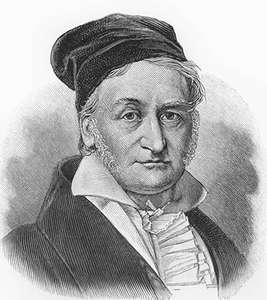
\includegraphics[width=0.8\linewidth]{figures/figure1}
    \caption{Some smart caption}\label{fig:example}
\end{figure}

\section{Some Math}
We can define scalar multiplication in $\mathbb{R}^n$ by
\begin{gather*}
    c[u_1,\dots,u_n] = [cu_1,\dots,cu_n]
\end{gather*}
You can now check that for $u,v\in\mathbb{R}^n$, we have
\begin{gather*}
	c(u+v)=cu+cv
\end{gather*}

% Backmatter
\cleardoublepage
% Probably you won't need to edit this file. Instead, edit the bib file itself.
\bibliographystyle{amsalpha}

\bibliography{thesis}
% The following command will make sure that the colophon is on an even page (the ``back'' of your thesis)
\cleardoubleevenpage
\thispagestyle{plain}
% Uncomment the addmargin environment when using Option 2 in the main file
% \begin{addmargin}[-0.6cm]{-3cm}

\hfill

\vfill


\pdfbookmark[0]{Colophon}{colophon}
\section*{Colophon}
\noindent This thesis was typeset using the typographical look-and-feel\\
\texttt{classicthesis} developed by Andr\'e Miede and Ivo Pletikosić.\bigskip

\noindent The style was inspired by Robert Bringhurst's seminal book\\
on typography ``\emph{The Elements of Typographic Style}''.\bigskip

\noindent Here you can insert things like ``Figures were created with...''\bigskip

\noindent [ Insert version number/description, if you want ]
% \end{addmargin}

\end{document}